%╔════════════════════════════╗
%║	  Szablon dostosował	  ║
%║	mgr inż. Dawid Kotlarski  ║
%║		  06.10.2024		  ║
%╚════════════════════════════╝
\documentclass[12pt,twoside,a4paper,openany]{article}

    % ------------------------------------------------------------------------
% PAKIETY
% ------------------------------------------------------------------------

%różne pakiety matematyczne, warto przejrzeć dokumentację, muszą być powyżej ustawień językowych.
\usepackage{mathrsfs}   %Różne symbole matematyczne opisane w katalogu ~\doc\latex\comprehensive. Zamienia \mathcal{L} ze zwykłego L na L-transformatę.
\usepackage{eucal}      %Różne symbole matematyczne.
\usepackage{amssymb}    %Różne symbole matematyczne.
\usepackage{amsmath}    %Dodatkowe funkcje matematyczne, np. polecenie \dfac{}{} skladajace ulamek w trybie wystawionym (porównaj $\dfrac{1}{2}$, a $\frac{1}{2}$).

%język polski i klawiatura
\usepackage[polish]{babel}
%\usepackage{qtimes} % czcionka Times new Roman
\usepackage[OT4]{polski}
%\usepackage[cp1250]{inputenc}                       %Strona kodowa polskich znaków.

%obsługa pdf'a
\usepackage[pdftex,usenames,dvipsnames]{color}      %Obsługa kolorów. Opcje usenames i dvipsnames wprowadzają dodatkowe nazwy kolorow.
\usepackage[pdftex,pagebackref=false,draft=false,pdfpagelabels=false,colorlinks=true,urlcolor=blue,linkcolor=black,citecolor=green,pdfstartview=FitH,pdfstartpage=1,pdfpagemode=UseOutlines,bookmarks=true,bookmarksopen=true,bookmarksopenlevel=2,bookmarksnumbered=true,pdfauthor={Dawid Kotlarski},pdftitle={Dokumentacja Projektowa},pdfsubject={},pdfkeywords={transient recovery voltage trv},unicode=true]{hyperref}   %Opcja pagebackref=true dotyczy bibliografii: pokazuje w spisie literatury numery stron, na których odwołano się do danej pozycji.

%bibliografia
%\usepackage[numbers,sort&compress]{natbib}  %Porządkuje zawartość odnośników do literatury, np. [2-4,6]. Musi być pod pdf'em, a styl bibliogfafii musi mieć nazwę z dodatkiem 'nat', np. \bibliographystyle{unsrtnat} (w kolejności cytowania).
\usepackage[
backend=biber,
style=numeric,
sorting=none
]{biblatex}
\addbibresource{bibliografia.bib}
\usepackage{hypernat}                       %Potrzebna pakietowi natbib do wspolpracy z pakietem hyperref (wazna kolejnosc: 1. hyperref, 2. natbib, 3. hypernat).

%grafika i geometria strony
\usepackage{extsizes}           %Dostepne inne rozmiary czcionek, np. 14 w poleceniu: \documentclass[14pt]{article}.
\usepackage[final]{graphicx}
\usepackage[a4paper,left=3.5cm,right=2.5cm,top=2.5cm,bottom=2.5cm]{geometry}

%strona tytułowa
\usepackage{strona_tytulowa}

%inne
\usepackage[hide]{todo}                     %Wprowadza polecenie \todo{treść}. Opcje pakietu: hide/show. Polecenie \todos ma byc na koncu dokumentu, wszystkie \todo{} po \todos sa ignorowane.
\usepackage[basic,physics]{circ}            %Wprowadza środowisko circuit do rysowania obwodów elektrycznych. Musi byc poniżej pakietow językowych.
\usepackage[sf,bf,outermarks]{titlesec}     %Troszczy się o wygląd tytułów rozdziałów (section, subsection, ...). sf oznacza czcionkę sans serif (typu arial), bf -- bold. U mnie: oddzielna linia dla naglowku paragraph. Patrz tez: tocloft -- lepiej robi format spisu tresci.
\usepackage{tocloft}                        %Troszczy się o format spisu trsci.
\usepackage{expdlist}    %Zmienia definicję środowiska description, daje większe możliwości wpływu na wygląd listy.
\usepackage{flafter}     %Wprowadza parametr [tb] do polecenia \suppressfloats[t] (polecenie to powoduje nie umieszczanie rysunkow, tabel itp. na stronach, na ktorych jest to polecenie (np. moze byc to stroma z tytulem rozdzialu, ktory chcemy zeby byl u samej gory, a nie np. pod rysunkiem)).
\usepackage{array}       %Ładniej drukuje tabelki (np. daje wiecej miejsca w komorkach -- nie są tak ścieśnione, jak bez tego pakietu).
\usepackage{listings}    %Listingi programow.
\usepackage[format=hang,labelsep=period,labelfont={bf,small},textfont=small]{caption}   %Formatuje podpisy pod rysunkami i tabelami. Parametr 'hang' powoduje wcięcie kolejnych linii podpisu na szerokosc nazwy podpisu, np. 'Rysunek 1.'.
\usepackage{appendix}    %Troszczy się o załączniki.
\usepackage{floatflt}    %Troszczy się o oblewanie rysunkow tekstem.
\usepackage{here}        %Wprowadza dodtkowy parametr umiejscowienia rysunków, tabel, itp.: H (duże). Umiejscawia obiekty ruchome dokladnie tam gdzie są w kodzie źródłowym dokumentu.
\usepackage{makeidx}     %Troszczy się o indeks (skorowidz).

%nieużywane, ale potencjalnie przydatne
\usepackage{sectsty}           %Formatuje nagłówki, np. żeby były kolorowe -- polecenie: \allsectionsfont{\color{Blue}}.
%\usepackage{version}           %Wersje dokumentu.

%============
\usepackage{longtable}			%tabelka
%============

%============
% Ustawienia listingów do kodu
%============

\usepackage{listings}
\usepackage{xcolor}

\definecolor{codegreen}{rgb}{0,0.6,0}
\definecolor{codegray}{rgb}{0.5,0.5,0.5}
\definecolor{codepurple}{rgb}{0.58,0,0.82}
\definecolor{backcolour}{rgb}{0.95,0.95,0.92}

% Definicja stylu "mystyle"
\lstdefinestyle{mystyle}{
	backgroundcolor=\color{backcolour},   
	commentstyle=\color{codegreen},
	keywordstyle=\color{blue},	%magenta
	numberstyle=\tiny\color{codegray},
	stringstyle=\color{codepurple},
	basicstyle=\ttfamily\footnotesize,
	breakatwhitespace=false,         
	breaklines=true,                 
	captionpos=b,                    
	keepspaces=true,                 
	numbers=left,                    
	numbersep=5pt,                  
	showspaces=false,                
	showstringspaces=false,
	showtabs=false,                  
	tabsize=2
}

\lstset{style=mystyle} % Deklaracja aktywnego stylu
%===========

%PAGINA GÓRNA I DOLNA
\usepackage{fancyhdr}          %Dodaje naglowki jakie się chce.
\pagestyle{fancy}
\fancyhf{}
% numery stron w paginie dolnej na srodku
\fancyfoot[C]{\scriptsize DOKUMENTACJA PROJEKTU - ZAAWANSOWANE PROGRAMOWANIE \\ 
\normalsize\sffamily  \thepage}


%\fancyhead[L]{\small\sffamily \nouppercase{\leftmark}}
\fancyhead[C]{\footnotesize \textit{AKADEMIA NAUK STOSOWANYCH W NOWYM SĄCZU}\\}

\renewcommand{\headrulewidth}{0.4pt}
\renewcommand{\footrulewidth}{0.4pt}

    % ------------------------------------------------------------------------
% USTAWIENIA
% ------------------------------------------------------------------------

% ------------------------------------------------------------------------
%   Kropki po numerach sekcji, podsekcji, itd.
%   Np. 1.2. Tytuł podrozdziału
% ------------------------------------------------------------------------
\makeatletter
    \def\numberline#1{\hb@xt@\@tempdima{#1.\hfil}}                      %kropki w spisie treści
    \renewcommand*\@seccntformat[1]{\csname the#1\endcsname.\enspace}   %kropki w treści dokumentu
\makeatother

% ------------------------------------------------------------------------
%   Numeracja równań, rysunków i tabel
%   Np.: (1.2), gdzie:
%   1 - numer sekcji, 2 - numer równania, rysunku, tabeli
%   Uwaga ogólna: o otoczeniu figure ma być najpierw \caption{}, potem \label{}, inaczej odnośnik nie działa!
% ------------------------------------------------------------------------
\makeatletter
    \@addtoreset{equation}{section} %resetuje licznik po rozpoczęciu nowej sekcji
    \renewcommand{\theequation}{{\thesection}.\@arabic\c@equation} %dodaje kropki

    \@addtoreset{figure}{section}
    \renewcommand{\thefigure}{{\thesection}.\@arabic\c@figure}

    \@addtoreset{table}{section}
    \renewcommand{\thetable}{{\thesection}.\@arabic\c@table}
\makeatother

% ------------------------------------------------------------------------
% Tablica
% ------------------------------------------------------------------------
\newenvironment{tabela}[3]
{
    \begin{table}[!htb]
    \centering
    \caption[#1]{#2}
    \vskip 9pt
    #3
}{
    \end{table}
}

% ------------------------------------------------------------------------
% Dostosowanie wyglądu pozycji listy \todos, np. zamiast 'p.' jest 'str.'
% ------------------------------------------------------------------------
\renewcommand{\todoitem}[2]{%
    \item \label{todo:\thetodo}%
    \ifx#1\todomark%
        \else\textbf{#1 }%
    \fi%
    (str.~\pageref{todopage:\thetodo})\ #2}
\renewcommand{\todoname}{Do zrobienia...}
\renewcommand{\todomark}{~uzupełnić}

% ------------------------------------------------------------------------
% Definicje
% ------------------------------------------------------------------------
\def\nonumsection#1{%
    \section*{#1}%
    \addcontentsline{toc}{section}{#1}%
    }
\def\nonumsubsection#1{%
    \subsection*{#1}%
    \addcontentsline{toc}{subsection}{#1}%
    }
\reversemarginpar %umieszcza notki po lewej stronie, czyli tam gdzie jest więcej miejsca
\def\notka#1{%
    \marginpar{\footnotesize{#1}}%
    }
\def\mathcal#1{%
    \mathscr{#1}%
    }
\newcommand{\atp}{ATP/EMTP} % Inaczej: \def\atp{ATP/EMTP}

% ------------------------------------------------------------------------
% Inne
% ------------------------------------------------------------------------
\frenchspacing                      
\hyphenation{ATP/-EMTP}             %dzielenie wyrazu w danym miejscu
\setlength{\parskip}{3pt}           %odstęp pomiędzy akapitami
\linespread{1.3}                    %odstęp pomiędzy liniami (interlinia)
\setcounter{tocdepth}{4}            %uwzględnianie w spisie treści czterech poziomów sekcji
\setcounter{secnumdepth}{4}         %numerowanie do czwartego poziomu sekcji 
\titleformat{\paragraph}[hang]      %wygląd nagłówków
{\normalfont\sffamily\bfseries}{\theparagraph}{1em}{}



    %polecenia zdefiniowane w pakiecie strona_tytulowa.sty
    \title{Szacowanie liczby pi za pomocą metody całkowania numerycznego całki oznaczonej, algorytm wielowątkowy}		%...Wpisać nazwę projektu...
    \author{Mateusz Stanek}
		
	\uczelnia{AKADEMIA NAUK STOSOWANYCH \\W NOWYM SĄCZU}
    \instytut{Wydział Nauk Inżynieryjnych}
    \kierunek{Katedra Informatyki}
    \praca{DOKUMENTACJA PROJEKTOWA}
    \przedmiot{ZAAWANSOWANE PROGRAMOWANIE}
    \prowadzacy{mgr inż. Dawid Kotlarski}
    \rok{2024}


%definicja składni mikrotik
\usepackage{fancyvrb}
\DefineVerbatimEnvironment{MT}{Verbatim}%
{commandchars=\+\[\],fontsize=\small,formatcom=\color{red},frame=lines,baselinestretch=1,} 
\let\mt\verb 
%zakonczenie definicji składni mikrotik

\usepackage{fancyhdr}    %biblioteka do nagłówka i stopki

			
\begin{document}
   
    \renewcommand{\figurename}{Rys.}    %musi byc pod \begin{document}, bo w~tym miejscu pakiet 'babel' narzuca swoje ustawienia
    \renewcommand{\tablename}{Tab.}     %j.w.
    \thispagestyle{empty}               %na tej stronie: brak numeru
    \stronatytulowa                     %strona tytułowa tworzona przez pakiet strona_tytulowa.tex
 
 \pagestyle{fancy}

    \newpage

    %formatowanie spisu treści i~nagłówków
    \renewcommand{\cftbeforesecskip}{8pt}
    \renewcommand{\cftsecafterpnum}{\vskip 8pt}
    \renewcommand{\cftparskip}{3pt}
    \renewcommand{\cfttoctitlefont}{\Large\bfseries\sffamily}
    \renewcommand{\cftsecfont}{\bfseries\sffamily}
    \renewcommand{\cftsubsecfont}{\sffamily}
    \renewcommand{\cftsubsubsecfont}{\sffamily}
    \renewcommand{\cftparafont}{\sffamily}
    %koniec formatowania spisu treści i nagłówków
     
    \tableofcontents    %spis treści
    \thispagestyle{fancy}
    \newpage

    
    \newpage

    
%%%%%%%%%%%%%%%%%%% treść główna dokumentu %%%%%%%%%%%%%%%%%%%%%%%%%

   	\newpage
\section{Ogólne określenie wymagań}		%1
%Określenie celu pracy, co chcemy uzyskać, jakie przewidujemy wyniki

\hspace{0.60cm}

Celem projektu jest utworzenie programu implementującego klasę Macierzy w języku \texttt{C++}. Jedak, głównym celem projektu jest zapoznanie się z narzędziem GitHub Copilot i wyrobienie sobie o nim opinii, dlatego program powinien być przez niego w dużej części napisany. 

Przewidywany jest działający program (w miarę możliwości modelu) i dokumentacja w Doxygenie.

   \newpage
\section{Analiza problemu}		%2
%Napisać gdzie używa się tego algorytmu
%Opisać sposób działania programu/algorytmu
%Napisać spsoób wykorzystania algorytmu po przez wykonanie przykładu (np. mnożenie macierzy - wykonać ręcznie przykład z mnożeniem macierzy pokazujący jak mnoży się macierz ręcznie)
%Jeśli zadanie zakłada przedstawienie jakiegoś narzędzia (np. git, AI) należy opisać narzędzie

\subsection{Algorytm obliczania $\pi$ metodą całkowania numerycznego}

Algorytm obliczania $\pi$ metodą całkowania numerycznego (połączenie metody Archimedesa\cite{archimedes} i sum Riemanna\cite{riemannwiki}) polega na wykorzystaniu wzoru na pole koła \[P = \pi r^2,\] Wzór ten można przekształcić do postaci \[\pi = \frac{P}{r^2},\] gdzie $P$ to pole koła, a $r$ to promień. Z tej relacji wynika, że można użyć wartości promienia i pola koła do obliczenia $\pi$. Jeżeli wiadomo jaki jest promień koła, do określenia pola pod łukiem ćwiartki okręgu i pomnożenia wyniku przez 4 (dlatego, że koło jest symetryczne względem osi $x$ i $y$ układu współrzędnych). Funkcję określająca kształt łuku ćwiartki można uzyskać poprzez przekształcenie wzoru okrąg \[x^2 + y^2 = r^2,\] gdzie $x$, $y$ to koordynaty punktów na okręgu, a $r$ to promień. Przekształcając wzór do postaci $f(x,r) \to y$ uzyskujemy \[y = \sqrt{r^2 - x^2},\] gdzie $y, x \geq 0$ (dlatego, że obliczana jest tylko ćwiartka). Pole pod tą funkcją to całka oznaczona \[P_{cw} = \int_{0}^{r} \sqrt{r^2 - x^2} \,dx.\] Pole całego koła to byłoby zatem \[P = 4P_{cw}.\]

Należy natomiast zauważyć, że nie da się obliczyć dokładnej wartości tej całki bez wykorzystania liczby $\pi$. Dlatego, należy skorzystać z sum Riemanna\cite{riemannwiki}, aby obliczyć aproksymację wartości $\pi$, poprzez podkładanie prostokątów z szerokością o danej wartości i wysokości określonej poprzez wartość funkcji $y = \sqrt{r^2 - x^2}$, gdzie $x$ to punkty oddzielone od siebie o daną szerokość.

\subsection{Git}
Kolejnym konceptem, którym zajmuje się projekt jest narzędzie git\cite{gitsite}. Pozwala ono zarządzać poszczególnymi wersjami projektów. Głównym korzeniem gita jest system commitów, czyli zapisania zmian w pliku w stosunku do commita starszego. To, w połączeniu z jego innymi możliwościami pozwala na tworzenie długich i skomplikowanych osi czasu danych projektów. 

Użycie gita można zademonstrować na prostym przykładzie. Tworzymy katalog a w nim repozytorium, uzywając komendy \texttt{git init}, jak widać na rys. \ref{fig:git_init}.

\begin{figure}[H]
	\centering
	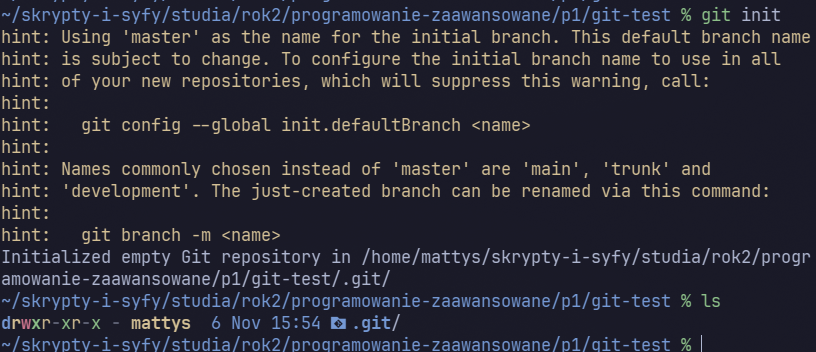
\includegraphics[width=1\textwidth]{images/git_init.png}
	\caption{\centering{Puste repozytorium git}}
	\label{fig:git_init}
\end{figure}

Stwórzmy jakiś plik i dodajmy go do repozytorium. Plik można dodać do repozytorium komendą \texttt{git add}

\begin{figure}[H]
	\centering
	
\includegraphics[width=1\textwidth]{images/git_add.png}
	\caption{\centering{Stworznie pliku w repozytorium}}
	\label{fig:git_add}
\end{figure}

Następnie należy scommitować zmiany. 

\begin{figure}[H]
	\centering
	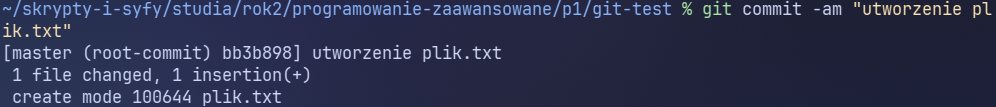
\includegraphics[width=1\textwidth]{images/git_commit1.png}
	\caption{\centering{Commit nr. 1}}
	\label{fig:git_commit1}
\end{figure}

Na rysunku \ref{fig:git_commit1} użyta komenda \texttt{git commit} commituje wszystkie dodane pliki (\texttt{-a}) z jakimś komunikatem (\texttt{-m}).  

\begin{figure}[H]
	\centering
	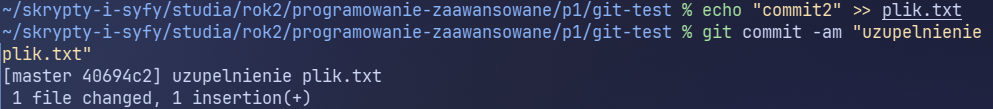
\includegraphics[width=1\textwidth]{images/git_commit2.png}
	\caption{\centering{Commit nr. 2}}
	\label{fig:git_commit2}
\end{figure}

Na rys. \ref{fig:git_commit2}, został utworzony kolejny commit, dodajacy zmiany do \texttt{plik.txt}.

\begin{figure}[H]
	\centering
	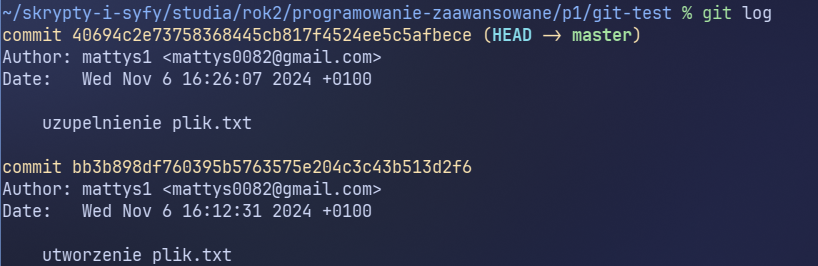
\includegraphics[width=1\textwidth]{images/git_log.png}
	\caption{\centering{Log gita}}
	\label{fig:git_log}
\end{figure}

Jak na rys. \ref{fig:git_log} jest pokazane, używając komendy \texttt{git log}, można wyświetlić log commitów w repozytorium.

\begin{figure}[H]
	\centering
	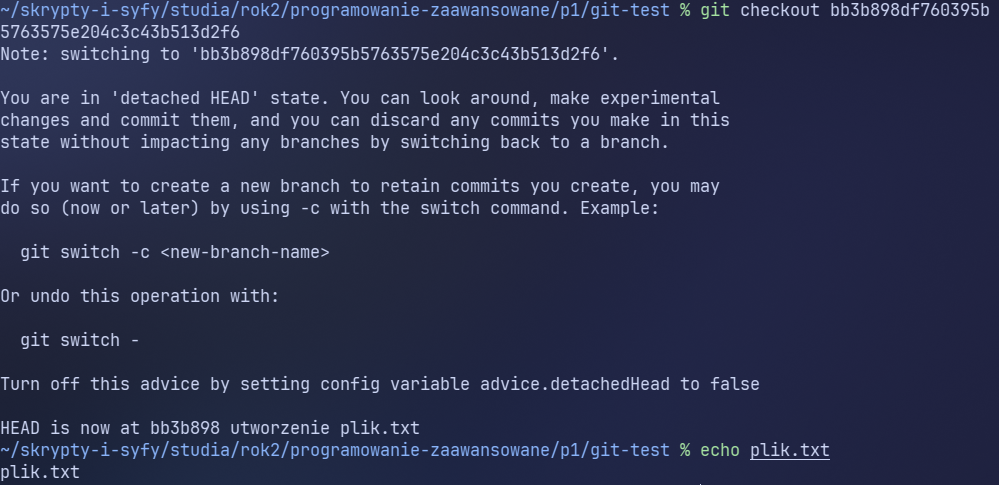
\includegraphics[width=1\textwidth]{images/git_checkout.png}
	\caption{\centering{Demonstracja checkout}}
	\label{fig:git_checkout}
\end{figure}

Jak widać na rys. \ref{fig:git_checkout}, komenda \texttt{git checkout}, pozwala na przejście repozytorium w inny stan, w tym przypadku przechodzi się do commita o danym ID, pokazanym na rys. \ref{fig:git_log}. Jako, że jest to pierwszy commit, nie ma w nim zmian z drugiego.

\subsection{Doxygen}
Doxygen\cite{doxygensite} jest narzędziem automatycznie generującym dokumentację programu z komentarzy w kodzie źródłowym. Potrafi on generować strony HTML, gdzie można dynamicznie nawigować się miedzy rożnymi częściami kodu oraz pliki \LaTeX, które można konwertować na różne, statyczne formaty.

\subsection{Github Copilot}

GitHub Copilot\cite{copilotsite} to model \texttt{LLM} oferowany przez GitHub - może on analizować kod źródłowy i funkcjonować jako zaawansowany autocompleter lub asystent potrafiący tworzyć proste fragmenty. Jest on bezpośrednio zintegrowany z wieloma narzędziami Microsoftu, takimi jak Visual Studio Code czy zwykłe Visual Studio. Jednak, jest on dostępny również jako rozszerzenie do innych edytorów, jak Neovim, którego instalacja przy użyciu menagera pluginów \texttt{Lazygit} jest ukazana na rys. \ref{fig:copilot_install}.

\begin{figure}[H]
	\centering
	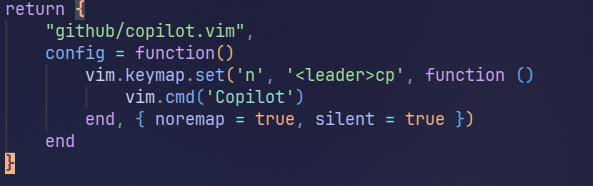
\includegraphics[width=1\textwidth]{images/copilot-plugin.png}
	\caption{\centering{Plik instalacyjny Plugina Copilot}}
	\label{fig:copilot_install}
\end{figure}

W Visual Studio jest on zainstalowany domyślnie.

\subsection{ChatGPT}

ChatGPT\cite{chatgptsite} jest serią modeli LLM oferowanych przez firmę OpenAI. W przeciwieństwie do Copilota jest on modelem bardziej skoncentrowanym na ogólnej tematyce, aniżeli na programowaniu. Jest on głównie nastawiony na funkcje czatu, ale oferowane jest też API do integracji z innymi narzędziami. 

\begin{figure}[H]
	\centering
	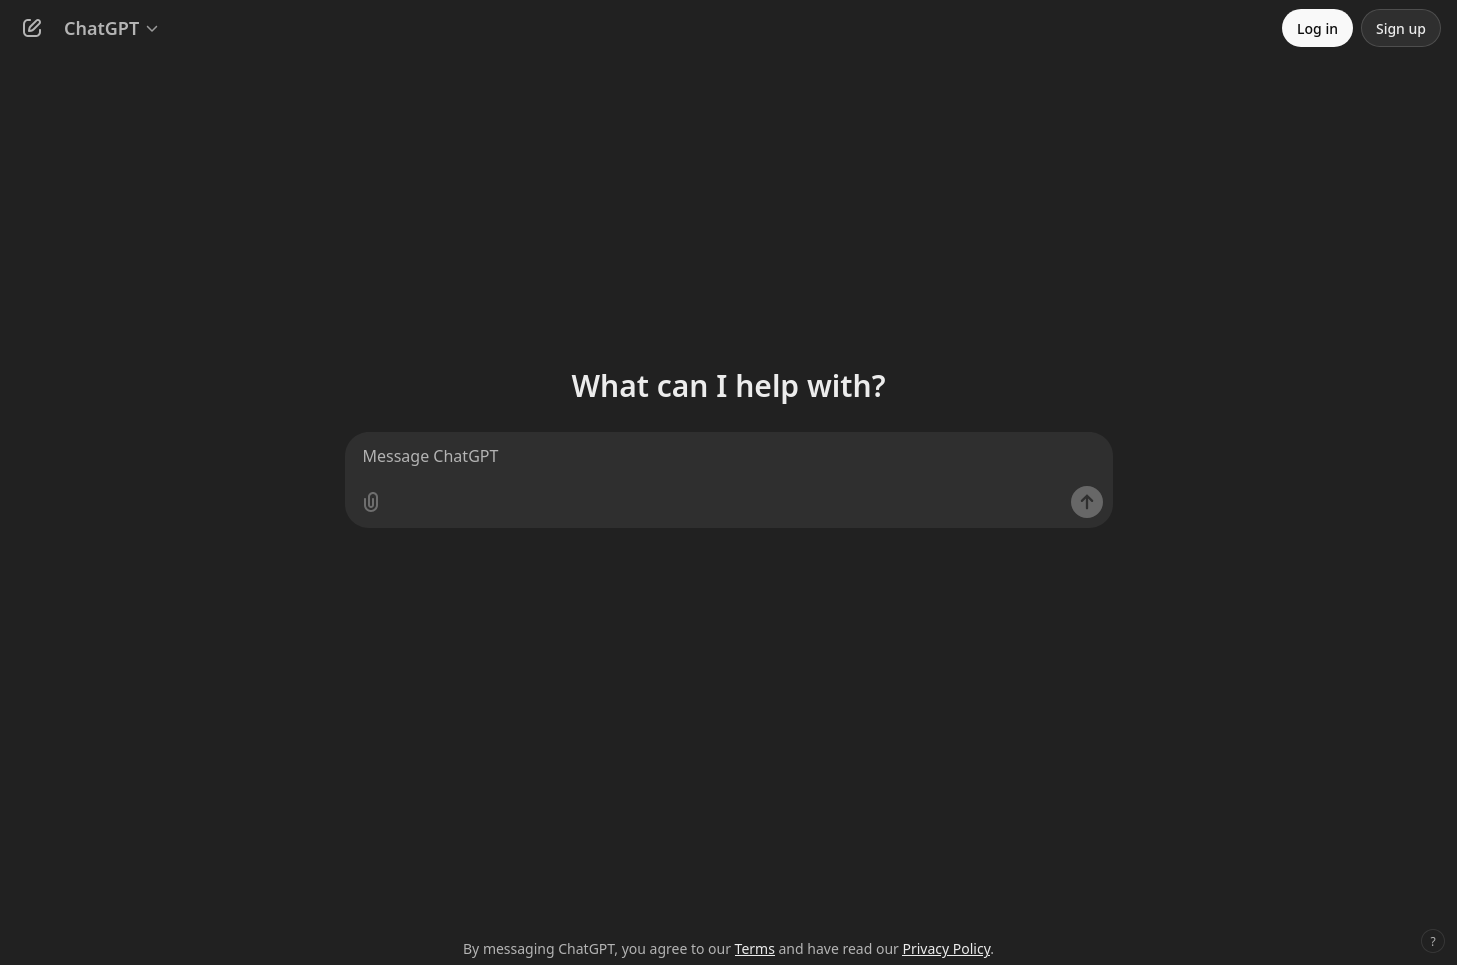
\includegraphics[width=1\textwidth]{images/chatgpt_site.png}
	\caption{\centering{Strona główna ChatGPT}}
	\label{fig:chatgptsite}
\end{figure}

   	\newpage
\section{Projektowanie}		%3
%Napisać z jakich narzędzi będziemy korzystać (kompilator, język programowania), git, biblioteki dodatkowe, itp.
%Opisać szczegółowe ustawienia kompilatora (jeśli są), powiązania z bibliotekami, itp.
%Narysować graf, UML, diagram klas, schemat działania algorytmu
%Jeśli zadanie zakłada przedstawienie jakiegoś narzędzia (np. git, AI) należy opisać sposób jego używania

\subsection{Implementacja macierzy}


Do zaimplementowania Macierzy zostanie użyty Język \texttt{C++} z kompilatorem \texttt{g++} oraz \texttt{MSVC}. Wersja standardu \texttt{C++} to \texttt{C++23}. Jako, że projekt ma być rozdzielony na dwa pliki, zostanie zastosowany \texttt{CMake} w celu automatyzacji procesu budowania. \texttt{CMake} pozwala na generowanie plików budujących dany projekt, zgodnie z określoną konfiguracją. Oszczędza to programiście, szczególnie przy większych projektach, manualne pisanie Makefileów.
Plik konfiguracyjny \texttt{CMakeLists.txt} może wyglądać jak na rysunku

\begin{lstlisting}[caption=Plik konfiguracyjny CMake, label={lst:cmakelists}, language=C++]
	cmake_minimum_required(VERSION 3.15)
	
	set(PROJECT_NAME proj4)
	
	project(${PROJECT_NAME} VERSION 0.1 LANGUAGES CXX)
	
	set(CMAKE_CXX_STANDARD 23)
	set(CMAKE_CXX_STANDARD_REQUIRED ON)
	set(CMAKE_EXPORT_COMPILE_COMMANDS True)
	set(CMAKE_RUNTIME_OUTPUT_DIRECTORY ${CMAKE_CURRENT_LIST_DIR}/out)
	
	add_subdirectory(src)
	
\end{lstlisting}

Edytorem będzie program Neovim oraz Visual Studio 2022 Community Edition. Jest to terminalowy edytor tekstu z możliwością poszerzenia funkcjonalności przy użyciu wszelkiego rodzaju pluginów. Wybrany został, dlatego że jest on już skonfigurowany na moim komputerze zgodnie z moimi preferencjami. Visual Studio jest zintegrowanym środowiskiem deweloperskim stworzonym i rozwijanym przez firmę Microsoft.

\subsection{Git}

Dla ułatwienia pracy, zastosowany został front-end dla gita o nazwie lazygit. Jest to terminalowy program, którego główną zaletą jest łatwa nawigacja przy użyciu klawiatury. Ponadto, jest on lekki i szybki.

\subsection{Doxygen}

Konfiguracja dla Doxygena jest wygenerowana przy użyciu programu doxywizard, pokazany na rys. \ref{fig:doxywizard}, pozwalającego na graficzne zmienianie ustawień. Po wygenerowaniu konfiguracji, Doxygen wywoływany jest przy użyciu komendy.

\begin{figure}[H]
	\centering
	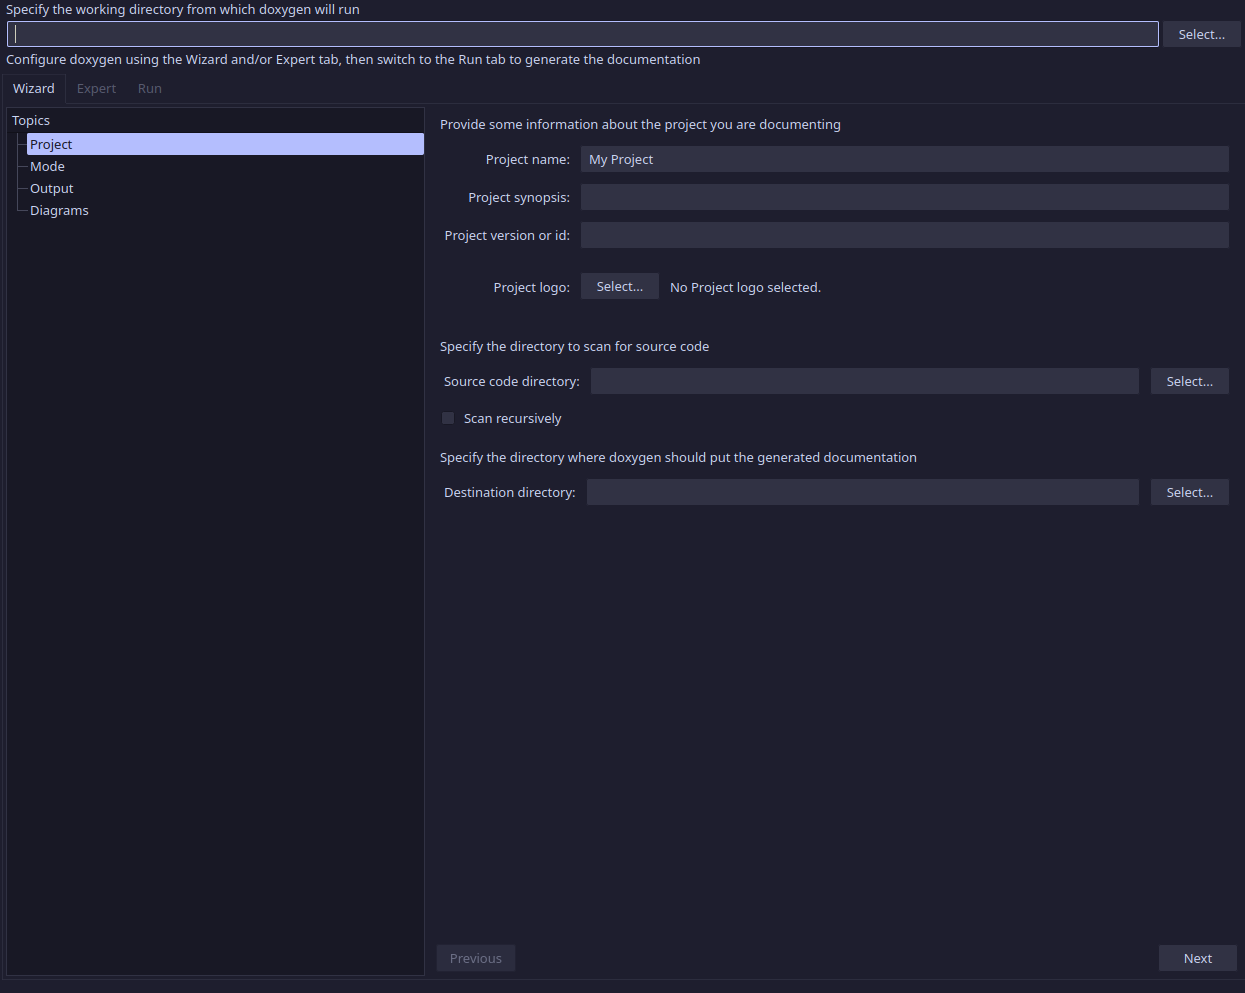
\includegraphics[width=1\textwidth]{images/doxywizard.png}
	\caption{\centering{Interfejs programu doxywizard}}
	\label{fig:doxywizard}
\end{figure}

\subsection{Github Copilot}
Do napisania programu do pomocy został wykorzystany Github Copilot. Z pomocy kopilota można skorzystać na 3 sposoby. Sposób pierwszy - poprzez podpowiedzi generowane przez copilota które są oznaczone kolorem szarym, co pokazano na rysunku nr \ref{fig:copilotsuggestion}.

\begin{figure}[H]
	\centering
	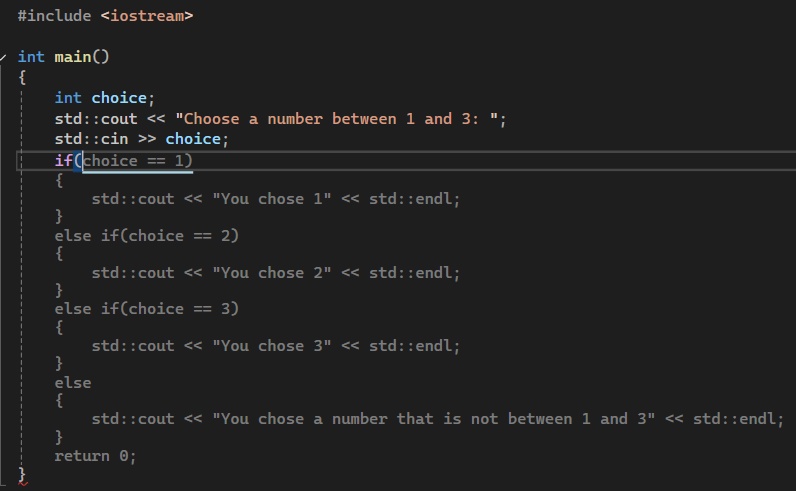
\includegraphics[width=1\linewidth]{images/CopilotSuggestion}
	\caption{\centering{Sugerowanie przez copilot}}
	\label{fig:copilotsuggestion}
\end{figure}

Sposób drugi to standardowe okienko chat gdzie można zapytać go o rzeczy związane z kodem, przedstawione zostało na rysunku nr \ref{fig:copilotchat}

\begin{figure}[H]
	\centering
	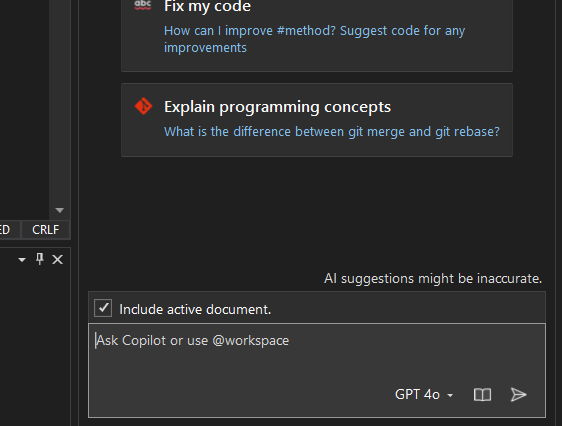
\includegraphics[width=1\linewidth]{images/CopilotChat}
	\caption{\centering{okienko chat Copilot}}
	\label{fig:copilotchat}
\end{figure}

Trzeci sposób to wykorzystanie komentarzy jako poleceń co ma zrobić copilot, jak pokazano na rysunku nr \ref{fig:copilotcomments}

\begin{figure}[H]
	\centering
	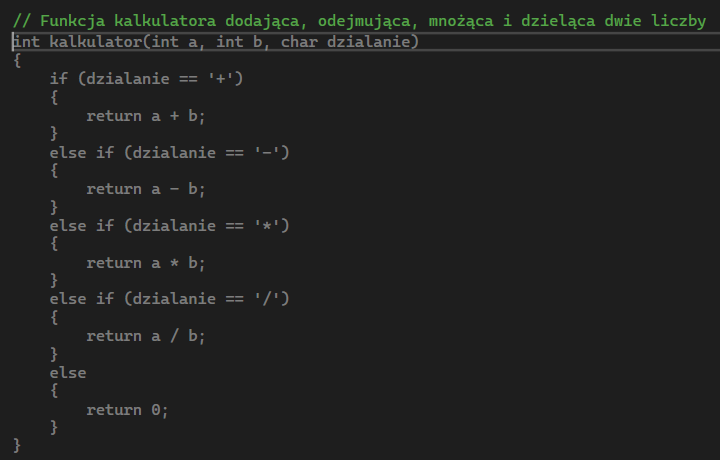
\includegraphics[width=1\linewidth]{images/CopilotComments}
	\caption{\centering{Zastosowanie komentarzy do generowania kodu}}
	\label{fig:copilotcomments}
\end{figure}

   	\newpage
\section{Implementacja}		%4
%Opisać implementacje algorytmu/programu. Pokazać ciekawe fragmenty kodu
%Opisać powstałe wyniki (algorytmu/nrzędzia)

\subsection{Klasa Matrix} \label{sec:Matrix}

Klasa jest zaimplementowana jako jeden plik \texttt{.hpp}. Nie jest podzielona na plik implementacji oraz nagłówek, ponieważ jest ona szablonem. Deklaracja klasy oraz prywatne elementy wyglądają tak jak na listingu nr.~\ref{lst:matrixclass}.

\begin{lstlisting}[caption=Klasa \texttt{Matrix}, label={lst:matrixclass}, language=C++]
	template <typename T>
	class Matrix {
		private:
		std::vector<std::vector<T>> data;
		
		public:
		
		Matrix(void) {}
		
		Matrix(int n) : data(n, std::vector<T>(n)) {}
		
		Matrix(int n, int* t) : data(n, std::vector<T>(n)) {
			for(auto& row : data){
				row = {t, t + n};
				t += n;
			}
		}
		
		Matrix(Matrix const& m) : data(m.data) {}
		
		void wypisz(void) {
			for(const auto& row : data){
				for(const auto& elem : row) {
					std::print("{} ", elem);
				}
				std::println();
			}
		}
		
		Matrix& alokuj(int n){
			if(data.size() == 0){
				data.resize(n, std::vector<T>(n));
			} else {
				if(data.size() < n){
					data.resize(n, std::vector<T>(n));
				}
			}
			return *this;
		}
		
		int pokaz(int x, int y) const {
			return data[x][y];
		}
		
		Matrix& dowroc(void) {
			Matrix<T> temp(data.size());
			
			for(int i = 0; i < data.size(); i++){
				for(int j = 0; j < data.size(); j++){
					temp.data[i][j] = data[j][i];
				}
			}
			
			*this = temp;
			return *this;
		}
		
		Matrix& losuj(void) {
			std::random_device rd;
			std::mt19937 gen(rd());
			std::uniform_int_distribution dis(0, 9);
			
			for(int i = 0; i < data.size(); i++){
				for(int j = 0; j < data.size(); j++){
					data[i][j] = dis(gen);
				}
			}
			return *this;
		}
		
		Matrix& losuj(int x) {
			if (data.size() == 0) return *this;
			
			std::random_device rd;
			std::mt19937 gen(rd());
			std::uniform_int_distribution<> dis(0, 9);
			
			int n = (int)data.size();
			for (int i = 0; i < x; i++) {
				int a = dis(gen) % n;
				int b = dis(gen) % n; // j.w.
				data[a][b] = dis(gen);
			}
			return *this;
		}
		
		Matrix& diagonalna(const int* t) {
			for(int i = 0; i < data.size(); i++){
				for(int j = 0; j < data.size(); j++){
					if(i == j){
						data[i][j] = t[i];
					} else {
						data[i][j] = 0;
					}
				}
			}
			return *this;
		}
		
		Matrix& diagonalna_k(int k, const int* t) {
			for(int i = 0; i < data.size(); i++){
				for(int j = 0; j < data.size(); j++){
					if(i == j + k){
						data[i][j] = t[j];
					} else {
						data[i][j] = 0;
					}
				}
			}
			return *this;
		}
		
		Matrix& kolumna(int x, const int* t) {
			for(int i = 0; i < data.size(); i++){
				data[i][x] = t[i];
			}
			return *this;
		}
		
		Matrix& wiersz(int x, const int* t) {
			for(int i = 0; i < data.size(); i++){
				data[x][i] = t[i];
			}
			return *this;
		}
		
		Matrix& przekatna(void) {
			for(int i = 0; i < data.size(); i++){
				for(int j = 0; j < data.size(); j++){
					if(i == j){
						data[i][j] = 1;
					} else {
						data[i][j] = 0;
					}
				}
			}
			return *this;
		}
		
		Matrix& pod_przekatna(void) {
			for(int i = 0; i < data.size(); i++){
				for(int j = 0; j < data.size(); j++){
					if(i > j){
						data[i][j] = 1;
					} else {
						data[i][j] = 0;
					}
				}
			}
			return *this;
		}
		
		Matrix& nad_przekatna(void) {
			for(int i = 0; i < data.size(); i++){
				for(int j = 0; j < data.size(); j++){
					if(i < j){
						data[i][j] = 1;
					} else {
						data[i][j] = 0;
					}
				}
			}
			return *this;
		}
		
		Matrix& wstaw(int x, int y, int wartosc) {
			data[x][y] = wartosc;
			return *this;
		}
		
		Matrix& szachownica(void) {
			for (int i = 0; i < (int)data.size(); i++) {
				for (int j = 0; j < (int)data.size(); j++) {
					data[i][j] = ((i + j) % 2 == 0) ? 0 : 1;
				}
			}
			return *this;
		}
		
		Matrix& operator+(Matrix const& m) {
			if (data.size() != m.data.size()) {
				return *this;
			}
			
			for (int i = 0; i < (int)data.size(); i++) {
				for (int j = 0; j < (int)data.size(); j++) {
					data[i][j] += m.data[i][j];
				}
			}
			return *this;
		}
		
		Matrix& operator*(Matrix const& m) {
			int n = (int)data.size();
			if (n == 0 || n != (int)m.data.size()) {
				return *this;
			}
			
			Matrix<T> result(n);
			for (int i = 0; i < n; i++) {
				for (int j = 0; j < n; j++) {
					T sum = 0;
					for (int k = 0; k < n; k++) {
						sum += data[i][k] * m.data[k][j];
					}
					result.data[i][j] = sum;
				}
			}
			*this = result;
			return *this;
		}
		
		Matrix& operator+(int a) {
			for (auto& row : data) {
				for (auto& elem : row) {
					elem += a;
				}
			}
			return *this;
		}
		
		Matrix& operator*(int a) {
			for (auto& row : data) {
				for (auto& elem : row) {
					elem *= a;
				}
			}
			return *this;
		}
		
		Matrix& operator-(int a) {
			for (auto& row : data) {
				for (auto& elem : row) {
					elem -= a;
				}
			}
			return *this;
		}
		
		friend Matrix operator+(int a, Matrix const& m) {
			Matrix result(m);
			for (auto& row : result.data) {
				for (auto& elem : row) {
					elem = a + elem;
				}
			}
			return result;
		}
		
		friend Matrix operator*(int a, Matrix const& m) {
			Matrix result(m);
			for (auto& row : result.data) {
				for (auto& elem : row) {
					elem = a * elem;
				}
			}
			return result;
		}
		
		friend Matrix operator-(int a, Matrix const& m) {
			Matrix result(m);
			for (auto& row : result.data) {
				for (auto& elem : row) {
					elem = a - elem;
				}
			}
			return result;
		}
		
		Matrix& operator++(int) {
			for (auto& row : data) {
				for (auto& elem : row) {
					elem += 1;
				}
			}
			return *this;
		}
		
		Matrix& operator--(int) {
			for (auto& row : data) {
				for (auto& elem : row) {
					elem -= 1;
				}
			}
			return *this;
		}
		
		Matrix& operator+=(int a) {
			for (auto& row : data) {
				for (auto& elem : row) {
					elem += a;
				}
			}
			return *this;
		}
		
		Matrix& operator-=(int a) {
			for (auto& row : data) {
				for (auto& elem : row) {
					elem -= a;
				}
			}
			return *this;
		}
		
		Matrix& operator*=(int a) {
			for (auto& row : data) {
				for (auto& elem : row) {
					elem *= a;
				}
			}
			return *this;
		}
		
		Matrix& operator()(double a) {
			int val = (int)std::floor(a);
			for (auto& row : data) {
				for (auto& elem : row) {
					elem += val;
				}
			}
			return *this;
		}
		
		friend std::ostream& operator<<(std::ostream& o, Matrix const& m) {
			for (const auto& row : m.data) {
				for (const auto& elem : row) {
					o << elem << " ";
				}
				o << "\n";
			}
			return o;
		}
		
		bool operator==(const Matrix& m) const {
			if (data.size() != m.data.size() || data[0].size() != m.data[0].size()) return false;
			for (int i = 0; i < (int)data.size(); i++) {
				for (int j = 0; j < (int)data[i].size(); j++) {
					if (data[i][j] != m.data[i][j]) return false;
				}
			}
			return true;
		}
		
		bool operator>(const Matrix& m) const {
			if (data.size() != m.data.size() || data[0].size() != m.data[0].size()) return false;
			for (int i = 0; i < (int)data.size(); i++) {
				for (int j = 0; j < (int)data[i].size(); j++) {
					if (!(data[i][j] > m.data[i][j])) return false;
				}
			}
			return true;
		}
		
		bool operator<(const Matrix& m) const {
			if (data.size() != m.data.size() || data[0].size() != m.data[0].size()) return false;
			for (int i = 0; i < (int)data.size(); i++) {
				for (int j = 0; j < (int)data[i].size(); j++) {
					if (!(data[i][j] < m.data[i][j])) return false;
				}
			}
			return true;
		}
	};
\end{lstlisting}
  
Klasa posiada tyko jedno prywatne pole, którym jest \texttt{std::vector<std::vector<T>> data}. oraz publiczne metody takie jak:
\begin{itemize}
	\item Konstruktor domyslny
	\item Konstruktor z rozmiarem macierzy
	\item 3 metody podstawowe, takie jak wypisz, alokuj, pokaz.
	\item Pozostałe metody
\end{itemize}
Metody zostaną opisane poniżej.

\begin{itemize}
    \item \texttt{wypisz()}\\
    Jest odpowiedzialna za wyświetlanie elementów macierzy w konsoli. Pętla zewnętrzna jest odpowiedzialna za przechodzenie przez wiersze macierzy a wewnętrzna przez elementy wiersza.

    \item \texttt{alokuj()}\\
    Jest odpowiedzialna za alokowanie pamięci dla macierzy o rozmiarze n*n. Jeżeli macierz jest pusta to tworzy nową macierz, jeżeli jest mniejsza od n to zmienia jej rozmiar na n*n.

    \item \texttt{pokaz()}\\
    Zwraca wartość elementu na pozycji x,y w macierzy.

    \item \texttt{dowroc()}\\
    Jest odpowiedzialna za zamianę wierszy z kolumnami. Tworzy tymczasową macierz \texttt{temp} aby wypełnić ją wartościami transponowanymi względem macierzy wejściowej. Następnie zastępuje bieżącą macierz nowymi wartościami.

    \item \texttt{losuj()}\\
    Tworzy generator liczb pseudolosowych od 0 do 9 a następnie przy pomocy pętli for wypełnia całą macierz losowymi wartościami z zakresu.

    \item \texttt{losuj\_x\_elementów()}\\
    Zasada działania jest podobna do poprzedniej metody losuj z zakresu ale tutaj losujemy x elementów.

    \item \texttt{szachownica()}\\
    Tworzy wzór szachownicy, gdzie pola mają wartość albo 0 albo 1, dzieje się to przy pomocy warunku (i+j) modulo 2 == 0.

    \item \texttt{porównania()}\\
    Sprawdza czy wszystkie elementy obu macierzy są równe.
\end{itemize}

   	\newpage
\section{Wnioski}	%5
%Npisać wnioski końcowe z przeprowadzonego projektu, 

\subsection{AI}
Nie należy ignorować narzędzi AI jak Copilot i uznawać je jako jakieś tymczasowe zabawki dla deweloperów, które kiedyś wyjdą z mody. Nawet w swoim obecnym stanie, sam fakt, że po napisaniu \texttt{for}, jednym kliknięciem taba, \textit{najprawdopodobniej} Copilot wytworzy nam sensowną pętle \textit{biorąc pod uwagę kontekst szerszego programu} jest bez dwóch zdań bardzo użyteczny, po prostu przez to, że oszczędza to programiście czas. Ponadto, narzędzia te są świetnymi wyszukiwarkami, co szczególnie się tyczy modeli, które mają dostęp do internetu. Nie trzeba praktycznie walczyć z zareklamowanym po kark Google i przeszukiwać napisanych przez boty stron - taki model automatycznie "przesieje" internet i pokaże nam informacje, które faktycznie dotyczą naszego zapytania. No, chyba że o to co się pytamy jest rzeczą niszową.

Niektórym (najbardziej to inwestorom w firmy zajmujące się AI) wydaje się, że LLM może za człowieka myśleć. Po części to prawda - jeżeli przed modelem o danym problemie myśleli inni - im więcej głowili się tym lepiej - i te przemyślenia gdzieś upublicznili, to LLM błyskawicznie może sięgnąć po tego problemu rozwiązanie. Ba, może nawet je po części zmodyfikować. Problem pojawia się, jeżeli zaczniemy naciskać na biednego chatbota. Fakty są następujące: LLM potrzebuje bardzo dużej ilości informacji o danym koncepcie, aby go opanować oraz LLM słabo potrafi rozumować, to jest, syntezować znane już informacje w nowe. Praktycznie, objawia się to gdy zapytamy się czatbota o rzecz, o której się mało mówi. 

Osobiście mogę przytoczyć przykład próby zrozumienia API \texttt{pipewire}\cite{pipewiresite}. Jest to projekt zajmujący się zarządzaniem strumieniami audio (takimi z aplikacji) na Linuxie. Rzecz, z natury niszowa. Chciałem przechwycić wyjście jednej aplikacji i uzyskać na bieżąco sample jakie wysyła. Ile to było bawienia się z ChatemGPT, prób wyplucia przez niego programu który się nie segfaultuje - głównie dlatego, że nie chciało mi się czytać dokumentacji. Czat podczas treningu pewnie przeczytał - ale mało co z tego wyciągnął, bo strona z API to było jedno z niewielu miejsc, gdzie owo API było opisane. W końcu okazało się, że na stronie był przykład programu, który robił prawie to samo co chciałem i jedyne co ChatGPT mi dał to powód do przeczytania dokumentacji. 

Pytać się można czy LLMy zastąpią programistów. Wydaje mi się, że - jeżeli nie teraz to za parę lat - programiści, których praca składa się z kopiowania zapytań o najnowszy framework JS ze Sack Overflowa i wklejania, faktycznie są zagrożeni, bo LLMy właściwie robią to, ale szybciej i taniej. Lecz programiści, którzy faktycznie tworzą coś nowego, faktycznie tworzą projekty wcześniej niedokonane, stoją na czele innowacji lub nią są - nie mają się czym martwić na długo.

Dotknąłem już do czego funkcja czatu może być użyteczna. W tym akurat zadaniu użyłem ChataGPT do pokazania faktycznej matematyki za algorytmem. Widać jego wypowiedź na rysunku nr.~\ref{fig:chatgptpcalka} 

\begin{figure}[H]
	\centering
	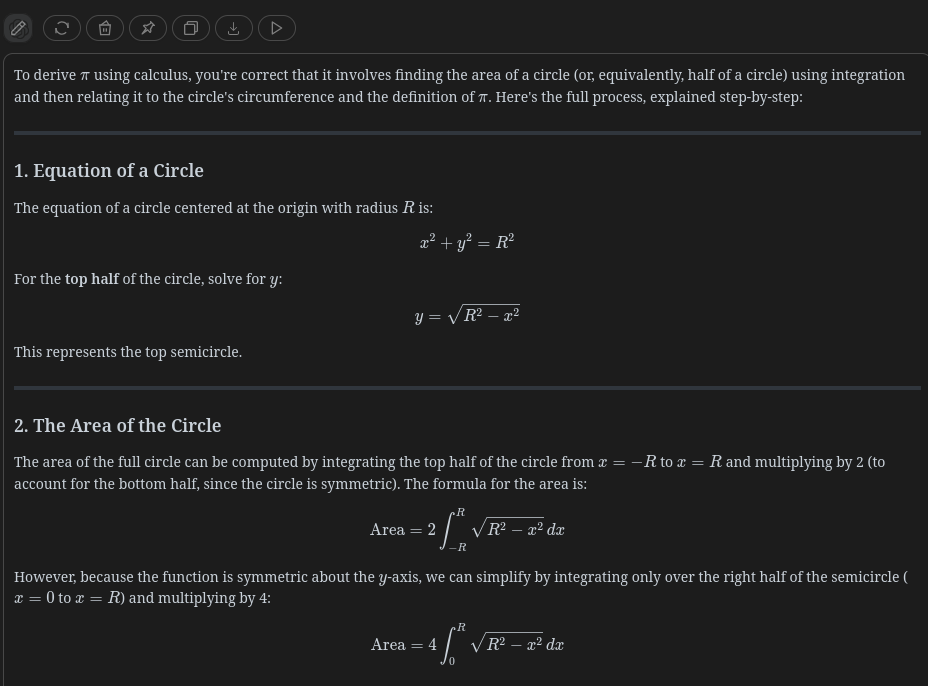
\includegraphics[width=1\textwidth]{images/chatgpt_calka.png}
	\caption{\centering{Wypowiedź Chata na temat sposobu obliczania pola pod kołem.}}
	\label{fig:chatgptpcalka}
\end{figure}

Wypowiedź z rysunku nr.~\ref{fig:chatgptpcalka} została wygenerowana modelem \texttt{gpt4o}.

\subsection{Wykonanie programu}

Program wykonuje się jak należy i kalkuluje $\pi$. Lecz warto zauważyć, że dla większej liczby wątków precyzja spada. Można to zauważyć na listingu nr. \ref{lst:accuracy}

\begin{lstlisting}[caption=Funkcja \texttt{getPi()}, label={lst:accuracy}, language=plaintext]
Select the accuracy of the algorithm (rectangles in a quarter of the circle): 10000000

Select the number of threads to use: 1

Calculated Pi: 3.141592853552536

------

Select the accuracy of the algorithm (rectangles in a quarter of the circle): 10000000

Select the number of threads to use: 50

Calculated Pi: 3.1415936525118267
\end{lstlisting}

Wartość $\pi$ to ok. $3.141592653589793$. Porównując 13 i ostatnią linijkę, dla 50 wątków, wartość $\pi$ jest mniej dokładna niż dla 1 wątku. Może to wynikać z tego, że wątki nie są synchronizowane, a więc mogą się zdarzyć przypadkowe kolizje, które zniekształcają wynik.

\subsection{Benchmarki}

Szersza implementacja benchmarków została opisana w sekcji nr.~\ref{sec:benchmarkimpl}. Benchmarki zostały przeprowadzone w dwóch zbiorach. Pierwszy, z wykresem na rysunku nr.~\ref{fig:benchmarklowc} pokrył zakres od 1 do \texttt{5'000'000'000} iteracji i 1 do 12 wątków (tyle jest na maszynie testującej). Drugi wykres którego jest zawarty na rysunku nr.~\ref{fig:benchmarkhighc}, testował od 1 do 50 wątków, ale ograniczony był do \texttt{1'000'000'000} iteracji, w celu oszczędzenia czasu. Osi \texttt{y} wykresów to suma wszystkich iteracji funkcji benchmarkującej dla danej ilości wątków. Oś \texttt{x} to po prostu ilość wątków użyta w benchmarku.

\begin{figure}[H]
	\centering
	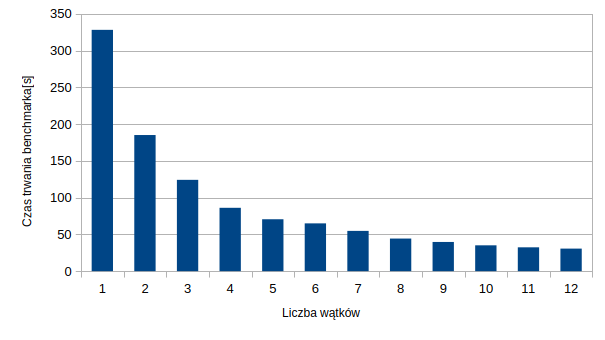
\includegraphics[width=1\textwidth]{images/benchmarks_lowc.png}
	\caption{\centering{Benchmark z niepełnym zakresem wątków}}
	\label{fig:benchmarklowc}
\end{figure}

\begin{figure}[H]
	\centering
	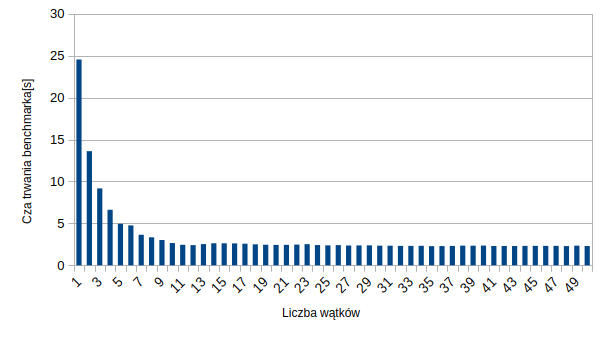
\includegraphics[width=1\textwidth]{images/benchmarks_highc.png}
	\caption{\centering{Benchmark z pełnym zakresem wątków}}
	\label{fig:benchmarkhighc}
\end{figure}

Jak widać na rysunku nr.~\ref{fig:benchmarklowc} wraz ze zwiększeniem liczby wątków, czas benchmarku zmniejsza się wykładniczo. Na rysunku nr. \ref{fig:benchmarkhighc} dzieje się podobnie, dopóki benchmark nie dojdzie do większej ilości wątków niż 12. Wtedy, czas wykonywania lekko wzrasta. Może się to dziać ponieważ tworzone jest więcej obiektów wątku, ale nie są one wykorzystywane przez procesor, co sprawia, że niepotrzebnie nakładany jest dodatkowy overhead.

   
       
%%%%%%%%%%%%%%%%%%% koniec treść główna dokumentu %%%%%%%%%%%%%%%%%%%%%
	\newpage
    \addcontentsline{toc}{section}{Literatura}  
	\printbibliography

    \newpage
    \hypersetup{linkcolor=black}
    \renewcommand{\cftparskip}{3pt}
    \clearpage
    \renewcommand{\cftloftitlefont}{\Large\bfseries\sffamily}
    \listoffigures
    \addcontentsline{toc}{section}{Spis rysunków}
	\thispagestyle{fancy}
	
    \newpage
    \renewcommand{\cftlottitlefont}{\Large\bfseries\sffamily}
    \def\listtablename{Spis tabel}
    \addcontentsline{toc}{section}{Spis tabel}\listoftables 
	\thispagestyle{fancy}
	
	\newpage
	\renewcommand{\cftlottitlefont}{\Large\bfseries\sffamily}
	\renewcommand\lstlistlistingname{Spis listingów}
	\addcontentsline{toc}{section}{Spis listingów}\lstlistoflistings 
	\thispagestyle{fancy}
	


    %lista rzeczy do zrobienia: wypisuje na koñcu dokumentu, patrz: pakiet todo.sty
    \todos
    %koniec listy rzeczy do zrobienia
\end{document}
